% Options for packages loaded elsewhere
\PassOptionsToPackage{unicode}{hyperref}
\PassOptionsToPackage{hyphens}{url}
\PassOptionsToPackage{dvipsnames,svgnames,x11names}{xcolor}
%
\documentclass[
  letterpaper,
  DIV=11,
  numbers=noendperiod]{scrartcl}

\usepackage{amsmath,amssymb}
\usepackage{iftex}
\ifPDFTeX
  \usepackage[T1]{fontenc}
  \usepackage[utf8]{inputenc}
  \usepackage{textcomp} % provide euro and other symbols
\else % if luatex or xetex
  \usepackage{unicode-math}
  \defaultfontfeatures{Scale=MatchLowercase}
  \defaultfontfeatures[\rmfamily]{Ligatures=TeX,Scale=1}
\fi
\usepackage{lmodern}
\ifPDFTeX\else  
    % xetex/luatex font selection
\fi
% Use upquote if available, for straight quotes in verbatim environments
\IfFileExists{upquote.sty}{\usepackage{upquote}}{}
\IfFileExists{microtype.sty}{% use microtype if available
  \usepackage[]{microtype}
  \UseMicrotypeSet[protrusion]{basicmath} % disable protrusion for tt fonts
}{}
\makeatletter
\@ifundefined{KOMAClassName}{% if non-KOMA class
  \IfFileExists{parskip.sty}{%
    \usepackage{parskip}
  }{% else
    \setlength{\parindent}{0pt}
    \setlength{\parskip}{6pt plus 2pt minus 1pt}}
}{% if KOMA class
  \KOMAoptions{parskip=half}}
\makeatother
\usepackage{xcolor}
\setlength{\emergencystretch}{3em} % prevent overfull lines
\setcounter{secnumdepth}{-\maxdimen} % remove section numbering
% Make \paragraph and \subparagraph free-standing
\ifx\paragraph\undefined\else
  \let\oldparagraph\paragraph
  \renewcommand{\paragraph}[1]{\oldparagraph{#1}\mbox{}}
\fi
\ifx\subparagraph\undefined\else
  \let\oldsubparagraph\subparagraph
  \renewcommand{\subparagraph}[1]{\oldsubparagraph{#1}\mbox{}}
\fi

\usepackage{color}
\usepackage{fancyvrb}
\newcommand{\VerbBar}{|}
\newcommand{\VERB}{\Verb[commandchars=\\\{\}]}
\DefineVerbatimEnvironment{Highlighting}{Verbatim}{commandchars=\\\{\}}
% Add ',fontsize=\small' for more characters per line
\usepackage{framed}
\definecolor{shadecolor}{RGB}{241,243,245}
\newenvironment{Shaded}{\begin{snugshade}}{\end{snugshade}}
\newcommand{\AlertTok}[1]{\textcolor[rgb]{0.68,0.00,0.00}{#1}}
\newcommand{\AnnotationTok}[1]{\textcolor[rgb]{0.37,0.37,0.37}{#1}}
\newcommand{\AttributeTok}[1]{\textcolor[rgb]{0.40,0.45,0.13}{#1}}
\newcommand{\BaseNTok}[1]{\textcolor[rgb]{0.68,0.00,0.00}{#1}}
\newcommand{\BuiltInTok}[1]{\textcolor[rgb]{0.00,0.23,0.31}{#1}}
\newcommand{\CharTok}[1]{\textcolor[rgb]{0.13,0.47,0.30}{#1}}
\newcommand{\CommentTok}[1]{\textcolor[rgb]{0.37,0.37,0.37}{#1}}
\newcommand{\CommentVarTok}[1]{\textcolor[rgb]{0.37,0.37,0.37}{\textit{#1}}}
\newcommand{\ConstantTok}[1]{\textcolor[rgb]{0.56,0.35,0.01}{#1}}
\newcommand{\ControlFlowTok}[1]{\textcolor[rgb]{0.00,0.23,0.31}{#1}}
\newcommand{\DataTypeTok}[1]{\textcolor[rgb]{0.68,0.00,0.00}{#1}}
\newcommand{\DecValTok}[1]{\textcolor[rgb]{0.68,0.00,0.00}{#1}}
\newcommand{\DocumentationTok}[1]{\textcolor[rgb]{0.37,0.37,0.37}{\textit{#1}}}
\newcommand{\ErrorTok}[1]{\textcolor[rgb]{0.68,0.00,0.00}{#1}}
\newcommand{\ExtensionTok}[1]{\textcolor[rgb]{0.00,0.23,0.31}{#1}}
\newcommand{\FloatTok}[1]{\textcolor[rgb]{0.68,0.00,0.00}{#1}}
\newcommand{\FunctionTok}[1]{\textcolor[rgb]{0.28,0.35,0.67}{#1}}
\newcommand{\ImportTok}[1]{\textcolor[rgb]{0.00,0.46,0.62}{#1}}
\newcommand{\InformationTok}[1]{\textcolor[rgb]{0.37,0.37,0.37}{#1}}
\newcommand{\KeywordTok}[1]{\textcolor[rgb]{0.00,0.23,0.31}{#1}}
\newcommand{\NormalTok}[1]{\textcolor[rgb]{0.00,0.23,0.31}{#1}}
\newcommand{\OperatorTok}[1]{\textcolor[rgb]{0.37,0.37,0.37}{#1}}
\newcommand{\OtherTok}[1]{\textcolor[rgb]{0.00,0.23,0.31}{#1}}
\newcommand{\PreprocessorTok}[1]{\textcolor[rgb]{0.68,0.00,0.00}{#1}}
\newcommand{\RegionMarkerTok}[1]{\textcolor[rgb]{0.00,0.23,0.31}{#1}}
\newcommand{\SpecialCharTok}[1]{\textcolor[rgb]{0.37,0.37,0.37}{#1}}
\newcommand{\SpecialStringTok}[1]{\textcolor[rgb]{0.13,0.47,0.30}{#1}}
\newcommand{\StringTok}[1]{\textcolor[rgb]{0.13,0.47,0.30}{#1}}
\newcommand{\VariableTok}[1]{\textcolor[rgb]{0.07,0.07,0.07}{#1}}
\newcommand{\VerbatimStringTok}[1]{\textcolor[rgb]{0.13,0.47,0.30}{#1}}
\newcommand{\WarningTok}[1]{\textcolor[rgb]{0.37,0.37,0.37}{\textit{#1}}}

\providecommand{\tightlist}{%
  \setlength{\itemsep}{0pt}\setlength{\parskip}{0pt}}\usepackage{longtable,booktabs,array}
\usepackage{calc} % for calculating minipage widths
% Correct order of tables after \paragraph or \subparagraph
\usepackage{etoolbox}
\makeatletter
\patchcmd\longtable{\par}{\if@noskipsec\mbox{}\fi\par}{}{}
\makeatother
% Allow footnotes in longtable head/foot
\IfFileExists{footnotehyper.sty}{\usepackage{footnotehyper}}{\usepackage{footnote}}
\makesavenoteenv{longtable}
\usepackage{graphicx}
\makeatletter
\def\maxwidth{\ifdim\Gin@nat@width>\linewidth\linewidth\else\Gin@nat@width\fi}
\def\maxheight{\ifdim\Gin@nat@height>\textheight\textheight\else\Gin@nat@height\fi}
\makeatother
% Scale images if necessary, so that they will not overflow the page
% margins by default, and it is still possible to overwrite the defaults
% using explicit options in \includegraphics[width, height, ...]{}
\setkeys{Gin}{width=\maxwidth,height=\maxheight,keepaspectratio}
% Set default figure placement to htbp
\makeatletter
\def\fps@figure{htbp}
\makeatother
\newlength{\cslhangindent}
\setlength{\cslhangindent}{1.5em}
\newlength{\csllabelwidth}
\setlength{\csllabelwidth}{3em}
\newlength{\cslentryspacingunit} % times entry-spacing
\setlength{\cslentryspacingunit}{\parskip}
\newenvironment{CSLReferences}[2] % #1 hanging-ident, #2 entry spacing
 {% don't indent paragraphs
  \setlength{\parindent}{0pt}
  % turn on hanging indent if param 1 is 1
  \ifodd #1
  \let\oldpar\par
  \def\par{\hangindent=\cslhangindent\oldpar}
  \fi
  % set entry spacing
  \setlength{\parskip}{#2\cslentryspacingunit}
 }%
 {}
\usepackage{calc}
\newcommand{\CSLBlock}[1]{#1\hfill\break}
\newcommand{\CSLLeftMargin}[1]{\parbox[t]{\csllabelwidth}{#1}}
\newcommand{\CSLRightInline}[1]{\parbox[t]{\linewidth - \csllabelwidth}{#1}\break}
\newcommand{\CSLIndent}[1]{\hspace{\cslhangindent}#1}

\KOMAoption{captions}{tableheading}
\makeatletter
\makeatother
\makeatletter
\makeatother
\makeatletter
\@ifpackageloaded{caption}{}{\usepackage{caption}}
\AtBeginDocument{%
\ifdefined\contentsname
  \renewcommand*\contentsname{Table of contents}
\else
  \newcommand\contentsname{Table of contents}
\fi
\ifdefined\listfigurename
  \renewcommand*\listfigurename{List of Figures}
\else
  \newcommand\listfigurename{List of Figures}
\fi
\ifdefined\listtablename
  \renewcommand*\listtablename{List of Tables}
\else
  \newcommand\listtablename{List of Tables}
\fi
\ifdefined\figurename
  \renewcommand*\figurename{Figure}
\else
  \newcommand\figurename{Figure}
\fi
\ifdefined\tablename
  \renewcommand*\tablename{Table}
\else
  \newcommand\tablename{Table}
\fi
}
\@ifpackageloaded{float}{}{\usepackage{float}}
\floatstyle{ruled}
\@ifundefined{c@chapter}{\newfloat{codelisting}{h}{lop}}{\newfloat{codelisting}{h}{lop}[chapter]}
\floatname{codelisting}{Listing}
\newcommand*\listoflistings{\listof{codelisting}{List of Listings}}
\makeatother
\makeatletter
\@ifpackageloaded{caption}{}{\usepackage{caption}}
\@ifpackageloaded{subcaption}{}{\usepackage{subcaption}}
\makeatother
\makeatletter
\@ifpackageloaded{tcolorbox}{}{\usepackage[skins,breakable]{tcolorbox}}
\makeatother
\makeatletter
\@ifundefined{shadecolor}{\definecolor{shadecolor}{rgb}{.97, .97, .97}}
\makeatother
\makeatletter
\makeatother
\makeatletter
\makeatother
\ifLuaTeX
  \usepackage{selnolig}  % disable illegal ligatures
\fi
\IfFileExists{bookmark.sty}{\usepackage{bookmark}}{\usepackage{hyperref}}
\IfFileExists{xurl.sty}{\usepackage{xurl}}{} % add URL line breaks if available
\urlstyle{same} % disable monospaced font for URLs
\hypersetup{
  pdftitle={Beyond PLSR: Bayesian Brilliance in Hyperspectral Trait Estimation},
  colorlinks=true,
  linkcolor={blue},
  filecolor={Maroon},
  citecolor={Blue},
  urlcolor={Blue},
  pdfcreator={LaTeX via pandoc}}

\title{Beyond PLSR: Bayesian Brilliance in Hyperspectral Trait
Estimation}
\author{}
\date{}

\begin{document}
\maketitle
\ifdefined\Shaded\renewenvironment{Shaded}{\begin{tcolorbox}[frame hidden, borderline west={3pt}{0pt}{shadecolor}, sharp corners, interior hidden, breakable, enhanced, boxrule=0pt]}{\end{tcolorbox}}\fi

\hypertarget{introduction}{%
\subsection{Introduction}\label{introduction}}

\begin{Shaded}
\begin{Highlighting}[]
\CommentTok{\# }\AlertTok{TODO}\CommentTok{: You can add other trait names from Roamresearch I.2{-}Paper{-}2}
\end{Highlighting}
\end{Shaded}

Foliar Functional traits are chemical (such as chlorophyll),
physiological (such as photosynthetic rate) and structural (such as leaf
area) features of a leaf which mediate ecosystem functioning and its
response to perturbations by regulating the growth fitness of plants in
diverse ecosystems (Serbin and Townsend (2020); Lavorel and Garnier
(2002); Wright et al. (2005); Funk et al. (2017)).

In an ecosystem, foliar functional traits influence the resource
allocation and reallocation of resources by a plant under diverse
environmental conditions ( Reich (2014); Wang et al. (2020)) and affect
the functional diversity driving ecosystem productivity ( Cadotte et al.
(2009) )

Foliar traits' significance in parameterizing terrestrial vegetation
plays a crucial role in Earth System models, which, if not precisely
characterized, introduces substantial uncertainty into climate change
predictions ( Wullschleger et al. (2014); Friedlingstein et al. (2006)
).

PLSR methods have been the most successful method for predicting traits
for spectra.\\
The upcoming SBG mission has PLSR method as one of the strong candidates
for predicting traits\\

The PLSR approach to trait estimation does not provide uncertainty
estimates which are crucial to understand how variable the predictions
will be when applied to new study regions.\\
Another drawback of the PLSR approach is that it assumes a linear
relationship between the traits and spectra. Though there have been a
few applications of kernel based PLSR approaches for trait prediction
(e.g. Arenas-Garcia and Camps-Valls (2008)) , the majority of the
studies still use the standard PLSR assuming a linear relationship
between the traits and spectra.\\
PLSR approaches also cannot account for the hierarchical structure that
might exist in certain traits.\\
PLSR is challenged by the variability of the relationship between traits
and spectra across species, functional types, and biomes. It will either
a global function between the traits and spectra which ignores the
across-group variability or else it is used to fit functions separately
for different groups which might not be always be possible due to
scarcity of sampled trait data.

The National Academy of Sciences 2017 Decadal Survey specifically
identifies the spatio-temporal distribution of plant functional traits
as a crucial objective (E-1a).\\
It is not surprising that plant functional traits are identified as an
Essential Biodiversity Variable (Pereira et al. (2013), Pettorelli et
al. (2016)).

\hypertarget{study-area-and-data}{%
\subsection{Study Area and Data}\label{study-area-and-data}}

We use observations of three foliar traits: Carotenoid
(\(\mu g/cm^{-2}\)), Nitrogen (\(mg/g\)) and Leaf Mass per Area
(\(g/m^{-2}\)) paired with hyperspectral reflectance data from 400 nm to
2400 nm from publicly available Ecological Spectral Information System
(EcoSIS) library (citation needed). The observation span a wide range of
climatic and geographic range ( Figure~\ref{fig-studyarea} ) .

\begin{figure}

{\centering 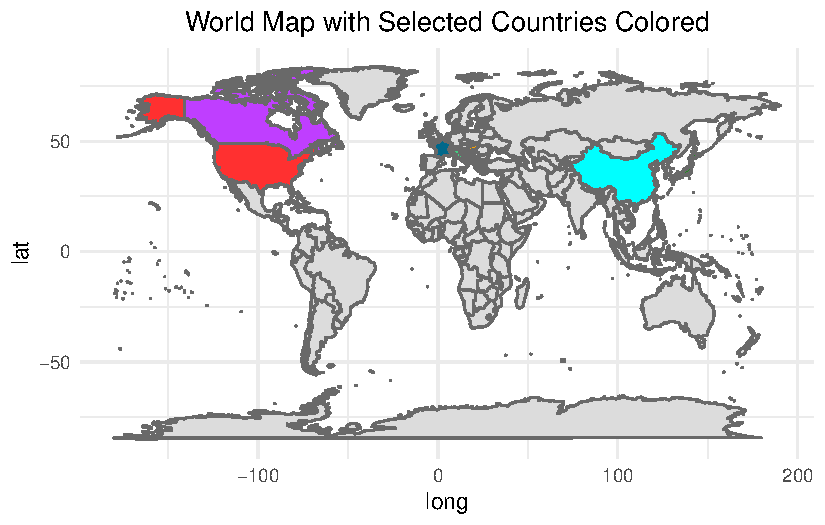
\includegraphics{paper_manuscript_files/figure-pdf/fig-studyarea-1.pdf}

}

\caption{\label{fig-studyarea}Study Area}

\end{figure}

\hypertarget{methods}{%
\subsection{Methods}\label{methods}}

In this section, we first describe the Bayesian regression model used in
predicting traits using hyperspectral data. We elucidate models both in
the actual spectral space as well as dimensionally reduced orthogonal
space (similar to PLSR). Formulating appropriate priors is essential for
high dimensional (where number of input spectral bands is large)
problems, therefore we also define the relevant priors used in the
current work. To enable computationally efficient prediction on new
datasets and select wavelengths which best approximate the predictive
capabilities of the above models, we transform both model to a simpler
model on the original spectral space requiring only a subset of input
spectra using projective inference (Juho Piironen, Markus Paasiniemi,
and Aki Vehtari 2020). Notationally, we denote a scalar with a lower
case letter and a vector with bold lower case letter. Superscript \(T\)
refers to transpose.

\hypertarget{data-processing}{%
\subsubsection{Data Processing}\label{data-processing}}

We downloaded and processed all spectra and trait data from EcoSIS so
that they have the same units across datasets.

The workflow for downloading and processing the data can be reproduced
by following the links to the Github page given in Appendix.

\hypertarget{bayesian-regression-model-original-hyperspectral-space}{%
\subsubsection{Bayesian Regression model-Original hyperspectral
space}\label{bayesian-regression-model-original-hyperspectral-space}}

Let the trait to be predicted be defined as a random variable \(y\). For
an \(i^{th}\) observation, let the measured trait value be defined as
\(y_i\) and the corresponding input (intercept plus) hyperspectral
wavelength be defined as the vector
\(\boldsymbol{x_i} = (1, x_{i,400}, x_{i,401}, ..., x_{i,2399}, x_{i,2400})\).
We assume that \(y_i\) is a linear function of \(\boldsymbol{x}\) such
that:

\(y_i = \boldsymbol{\beta}^T \boldsymbol{x_i} + \epsilon_i, \; \epsilon \sim N(0, \sigma^2), \; i = 1,..., n\)

where \(n\) is the number of observations.\\
Here the dimension of \(x_i\) is \(p = 2002\). \(\boldsymbol{\beta}\)
denotes the corresponding regression coefficients for
\(\boldsymbol{x_i}\), and \(\sigma^2\) is the noise variance. Let the
training data for the regression model i.e.~the \(n\) observations of
both the trait and spectra be denoted by \(\mathcal{D}\).

\hypertarget{formulating-priors}{%
\paragraph{Formulating priors}\label{formulating-priors}}

An important component of the Bayesian approach is to formulate
appropriate priors for the parameter vector
\(\boldsymbol{\theta} :=(\boldsymbol{\beta}, \sigma^{2})\) used in the
model.\\
Since the dimension of \(\boldsymbol{\beta}\) (2002) is large and a
functional trait is typically sensitive to a small subset of the
wavelengths, using traditionally used priors for \(\boldsymbol{\beta}\)
(such as normally distributed priors) can lead to over-fitting of the
Bayesian model.\\
This is especially true when the number of observations in
\$\textbackslash mathcal\{D\}\$ is less than \$p = 2002\$.\\
Since, a given trait is sensitive to a small number of wavelengths, we
need a prior distribution which shrinks the \$\textbackslash beta\$
coefficients of the non-important wavelengths to zero while letting the
regression coefficients of the important wavelengths escape this
shrinkage.\\
Such a prior distribution should therefore assign a high probability
density at zero while also have heavy-tail (which allows the modeling of
large values of \$\textbackslash beta\$) fo important wavelengths.\\
To achieve this, we use a special prior distribution for \(\beta_j\)
called the regularized horseshoe prior (Piironen and Vehtari 2017).\\
The regularized horseshoe prior belongs to a class of priors called
shrinkage or sparsifiying priors which shrink \(\beta\) coefficients of
the non-important wavelengths to zero and also have heavy-tails. For
\(j^{th}\) regresssion coefficient \(\beta_j\), the regularized horsehoe
prior is defined as:

\[
\begin{aligned}
& \beta_j|\lambda_j, \tau, c \sim N(0, \tau^2 \xi_j^2), \; \xi_j^2 = \frac{c^2\lambda_j^2} {c^2 + \tau^2\lambda_j^2 \\
& \lambda_j \sim C^+(0, 1), j = 1,..., p
\end{aligned}
\]

\(\beta_j|\lambda_j, \tau, c \sim N(0, \tau^2 \xi_j^2), \; \xi_j^2 = \frac{c^2\lambda_j^2} {c^2 + \tau^2\lambda_j^2}\),

\(\lambda_j \sim C^+(0, 1), j = 1,..., p\)

\(c^2 \sim Inv-Gamma (\nu, s^2)\)

where \(C^+\) is a standard half-Cauchy distribution on the positive
reals.\\
It is an extension of the horseshoe prior (Carvalho, Polson, and Scott
2010) which has been widely used in high-dimensional regression.\\
Similar to the horseshoe prior, the \(\tau\) parameter in regularized
horseshoe prior drives all regression coefficients to zero.\\
The thick Cauchy-tails for \(\lambda_j\) allow some of the regression
coefficients to escape this shrinkage towards zero.\\
The regularized horsehoe has an extra parameter \(c\) which better
penalizes the non-shrinkage coefficients (i.e.~the regression
coefficients that are not equal to zero).\\
This helps if the regression coefficients are weakly identified and also
speeds up the sampling during posterior parameter inference using Markov
Chain Monte Carlo (MCMC) methods.\\
The regularized horseshoe prior also incorporates our prior guess on the
number of wavelengths with non-zero regression coefficients.\\

\begin{figure}

{\centering 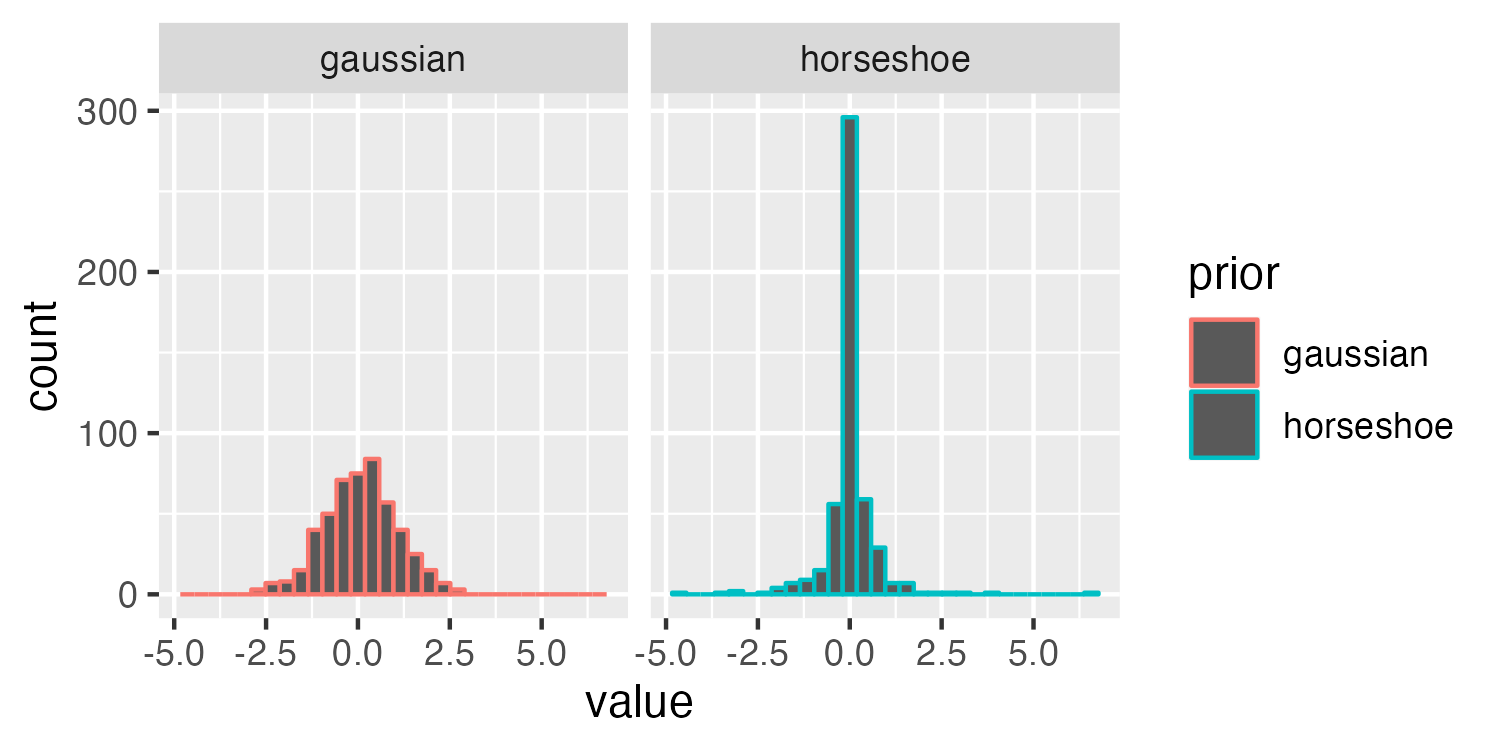
\includegraphics{paper_draft/figures/horseshoe_vs_gaussian.png}

}

\caption{\label{fig-method_horseshoe_vs_gaussian}Gaussian prior vs
Regularized horseshoe prior}

\end{figure}

\begin{Shaded}
\begin{Highlighting}[]
\CommentTok{\# Uncomment below if you want to plot the horseshoe vs gaussian prior simulations}
\CommentTok{\# library(extraDistr)}
\CommentTok{\# library(ggplot2)}
\CommentTok{\# m\_eff \textless{}{-} 0.05}
\CommentTok{\# nu \textless{}{-} 4}
\CommentTok{\# s = 2}
\CommentTok{\# n\_sim \textless{}{-} 500}
\CommentTok{\# }
\CommentTok{\# set.seed(100)}
\CommentTok{\# \# simulating from regularized horseshoe}
\CommentTok{\# beta\_j \textless{}{-} vector()}
\CommentTok{\# for(i in 1: n\_sim)}
\CommentTok{\# \{}
\CommentTok{\#   sigma = 1}
\CommentTok{\#   tau\_0\_sq \textless{}{-} m\_eff *sigma}
\CommentTok{\#   tau\_sq \textless{}{-} rhcauchy(n = 1, sigma = tau\_0\_sq)}
\CommentTok{\#   }
\CommentTok{\#   lambda\_j \textless{}{-} rhcauchy(n = 1, sigma = 1)}
\CommentTok{\#   }
\CommentTok{\#   alpha = nu/2; beta \textless{}{-} (nu *s\^{}2)/2}
\CommentTok{\#   c\_sq \textless{}{-} rinvgamma(n = 1, alpha = alpha, beta = beta)}
\CommentTok{\#   }
\CommentTok{\#   lambda\_j\_tilde\_sq \textless{}{-} (c\_sq * lambda\_j\^{}2)/(c\_sq + tau\_sq *lambda\_j\^{}2)}
\CommentTok{\#   beta\_j[i] \textless{}{-} rnorm(1, mean = 0, sd = sqrt(tau\_sq * lambda\_j\_tilde\_sq))}
\CommentTok{\# \}}
\CommentTok{\# hist(beta\_j, 1e4, freq = FALSE, col = "red")}
\CommentTok{\# \# simulating from normal distribution}
\CommentTok{\# }
\CommentTok{\# sigma = 0.05}
\CommentTok{\# beta\_j\_normal \textless{}{-} rnorm(n\_sim, sigma)}
\CommentTok{\# hist(beta\_j\_normal, 1e4, freq = FALSE, col = "red")}
\CommentTok{\# }
\CommentTok{\# \#\#make plot using ggplot}
\CommentTok{\# }
\CommentTok{\# beta\_df \textless{}{-} data.frame(value =  c(beta\_j, beta\_j\_normal), }
\CommentTok{\#                       prior = rep(c("horseshoe", "gaussian"), each = n\_sim))}
\CommentTok{\#                       }
\CommentTok{\# }
\CommentTok{\# ggplot(beta\_df, aes(x = value, color = prior)) + geom\_histogram() +}
\CommentTok{\# \#geom\_freqpoly(linewidth = 0.5) + }
\CommentTok{\#   facet\_wrap(\textasciitilde{}prior) }
\CommentTok{\# }
\CommentTok{\# ggsave(filename = "paper\_draft/figures/horseshoe\_vs\_gaussian.png",}
\CommentTok{\#        height = 2.5,}
\CommentTok{\#        width = 5,}
\CommentTok{\#        units = "in")}
\end{Highlighting}
\end{Shaded}

\hypertarget{bayesian-regression-model-dimensionally-reduced-orthogonal-space}{%
\subsubsection{Bayesian Regression model-dimensionally reduced
orthogonal
space}\label{bayesian-regression-model-dimensionally-reduced-orthogonal-space}}

\#\#Add text about bayesian supervised principal components\#\#

\hypertarget{model-reduction-in-original-spectral-space}{%
\subsubsection{Model reduction in original spectral
space}\label{model-reduction-in-original-spectral-space}}

The two models in the previous approach were designed to give good
predictions even if the model has redundant wavelengths as input. While
the model in Section M.1 has high computational cost, model in Section
M.2 loses interpretability due to projection of spectra into orthogonal
latent dimensions. We want our predictive model to be (a)
computationally fast when predicting new data, (b) interpretable and (c)
be able to account for uncertainties in the input wavelengths. A direct
way to achieve the above three objectives is to define a model which
takes a relevant subset of the hyperspectral wavelengths as input
(satisfying (a) and (c)) and does not do any transformation of input
wavelengths (satisfying (b)) while still predicting comparably to the
full model on new datasets.

Therefore, our aim is to find a reduced model such that

\(y_i = \boldsymbol{\beta_{*}^T} \boldsymbol{x_{i*}} + \epsilon_i, \; \epsilon \sim N(0, \sigma^2), \; i = 1,..., n\)

such that \(|\boldsymbol{x_i*}| = p_{*} << \boldsymbol{x_i} = p =2002\)
where \(|\boldsymbol{a}|\) denotes the length of a vector
\(\boldsymbol{a}\). Note that, in this work our aim is not to find all
wavelengths that are statistically related to the trait, but instead are
only focused on finding a minimal subset of wavelengths that give a good
predictive model for the given trait such that adding more wavelengths
to the model will not significantly improve the predictive accuracy
(Juho Piironen, Markus Paasiniemi, and Aki Vehtari 2020).

\hypertarget{posterior-projection-of-full-model}{%
\paragraph{Posterior projection of full
model}\label{posterior-projection-of-full-model}}

To formulate the reduced model, we use posterior projection (Juho
Piironen, Markus Paasiniemi, and Aki Vehtari 2020), which consists of
replacing the posterior distribution of the parameters of the full model
--e.g.~\(\boldsymbol{\theta}\) of the Bayesian regression model in
Section M.1-- with a simpler distribution \(q(\theta_{*}\)). The full
model is also called the reference model and we denote posterior
distribution of its parameters as
\(p(\boldsymbol{\theta}|\mathcal{D})\), where \(\mathcal{D}\) is the
training data. For the reference model in Section M.1, restricting the
model means setting some regression coefficients in
\(\boldsymbol{\beta}\) in the reference model equal to zero. For
supervised PC (Section M.3), since the reference model is now in the
latent orthogonal space, the projection works a bit differently since
the input variables in the reference model and the reduced model
(original spectral scale) are not similar. Therefore, to make the method
model agnostic, posterior projection is defined in terms of the loss in
posterior predictive accuracy --in terms of the Kullback-Liebler or KL
divergence-- when the reduced model is used in place of the reference
model. Specifically,

\(KL(p(\tilde{y}|\mathcal{D}) || q(\tilde{y}) ) = E_{\tilde{y}}(log(p(\tilde{y}|\mathcal{D})) - log(q(\tilde{y})))\)

We use the `tilde' notation to denote future measurements of the trait,
hence \(\tilde{y}\) denotes future measurement of the trait . Here,
\(p(\tilde{y}|\mathcal{D})\) is the posterior predictive distribution of
future measurements of the trait given the training data \(\mathcal{D}\)
for the reference model, \(q(\tilde{y})\) is the distribution of
\(\tilde{y}\) from the reduced model, \(E_{\tilde{y}}\) means the
expectation over all possible future measurements of the trait.The
objective of the posterior projection approach is to find the reduced
model \(q(\theta_{*})\) that minimizes equation ().

In our case, we will use the posterior projection to determine the
complexity (i.e the number of input wavelengths to be used) of our
linear spectral model. There are various ways to empirically find the
reduced model including draw-by-draw approach (GOUTIS and ROBERT 1998),
(Dupuis and Robert 2003) and the single point approach (Tran, Nott, and
Leng 2012). Here we use the clustered projection approach by (Juho
Piironen, Markus Paasiniemi, and Aki Vehtari 2020) which can be thought
of as a unification of the above-mentioned approaches and gives a nice
tradeoff between speed and accuracy.

Equation () gives us the optimal model for a given complexity i.e.~for a
given number of input wavelengths \(p_*\). To determine the minimum
value of \(p_*\), we compare the predictive utility of the reference
model and the set of reduced models for each \(p_*\) over a validation
set. Since we are working in a Bayesian framework, we choose the mean
log predictive density (MLPD) as our predictive utility function as it
not only compares the point predictions but also the predictive
uncertainties associated with the reduced model. This gives MLPD a
significant advantage over commonly used utility functions such as mean
squared error (MSE). For the validation set, we use K-fold cross
validation, fitting and validating the reduced model K times to avoid
over fitting.

The entire methodology is summarized in
Figure~\ref{fig-method_flowchart} :

\begin{figure}

{\centering 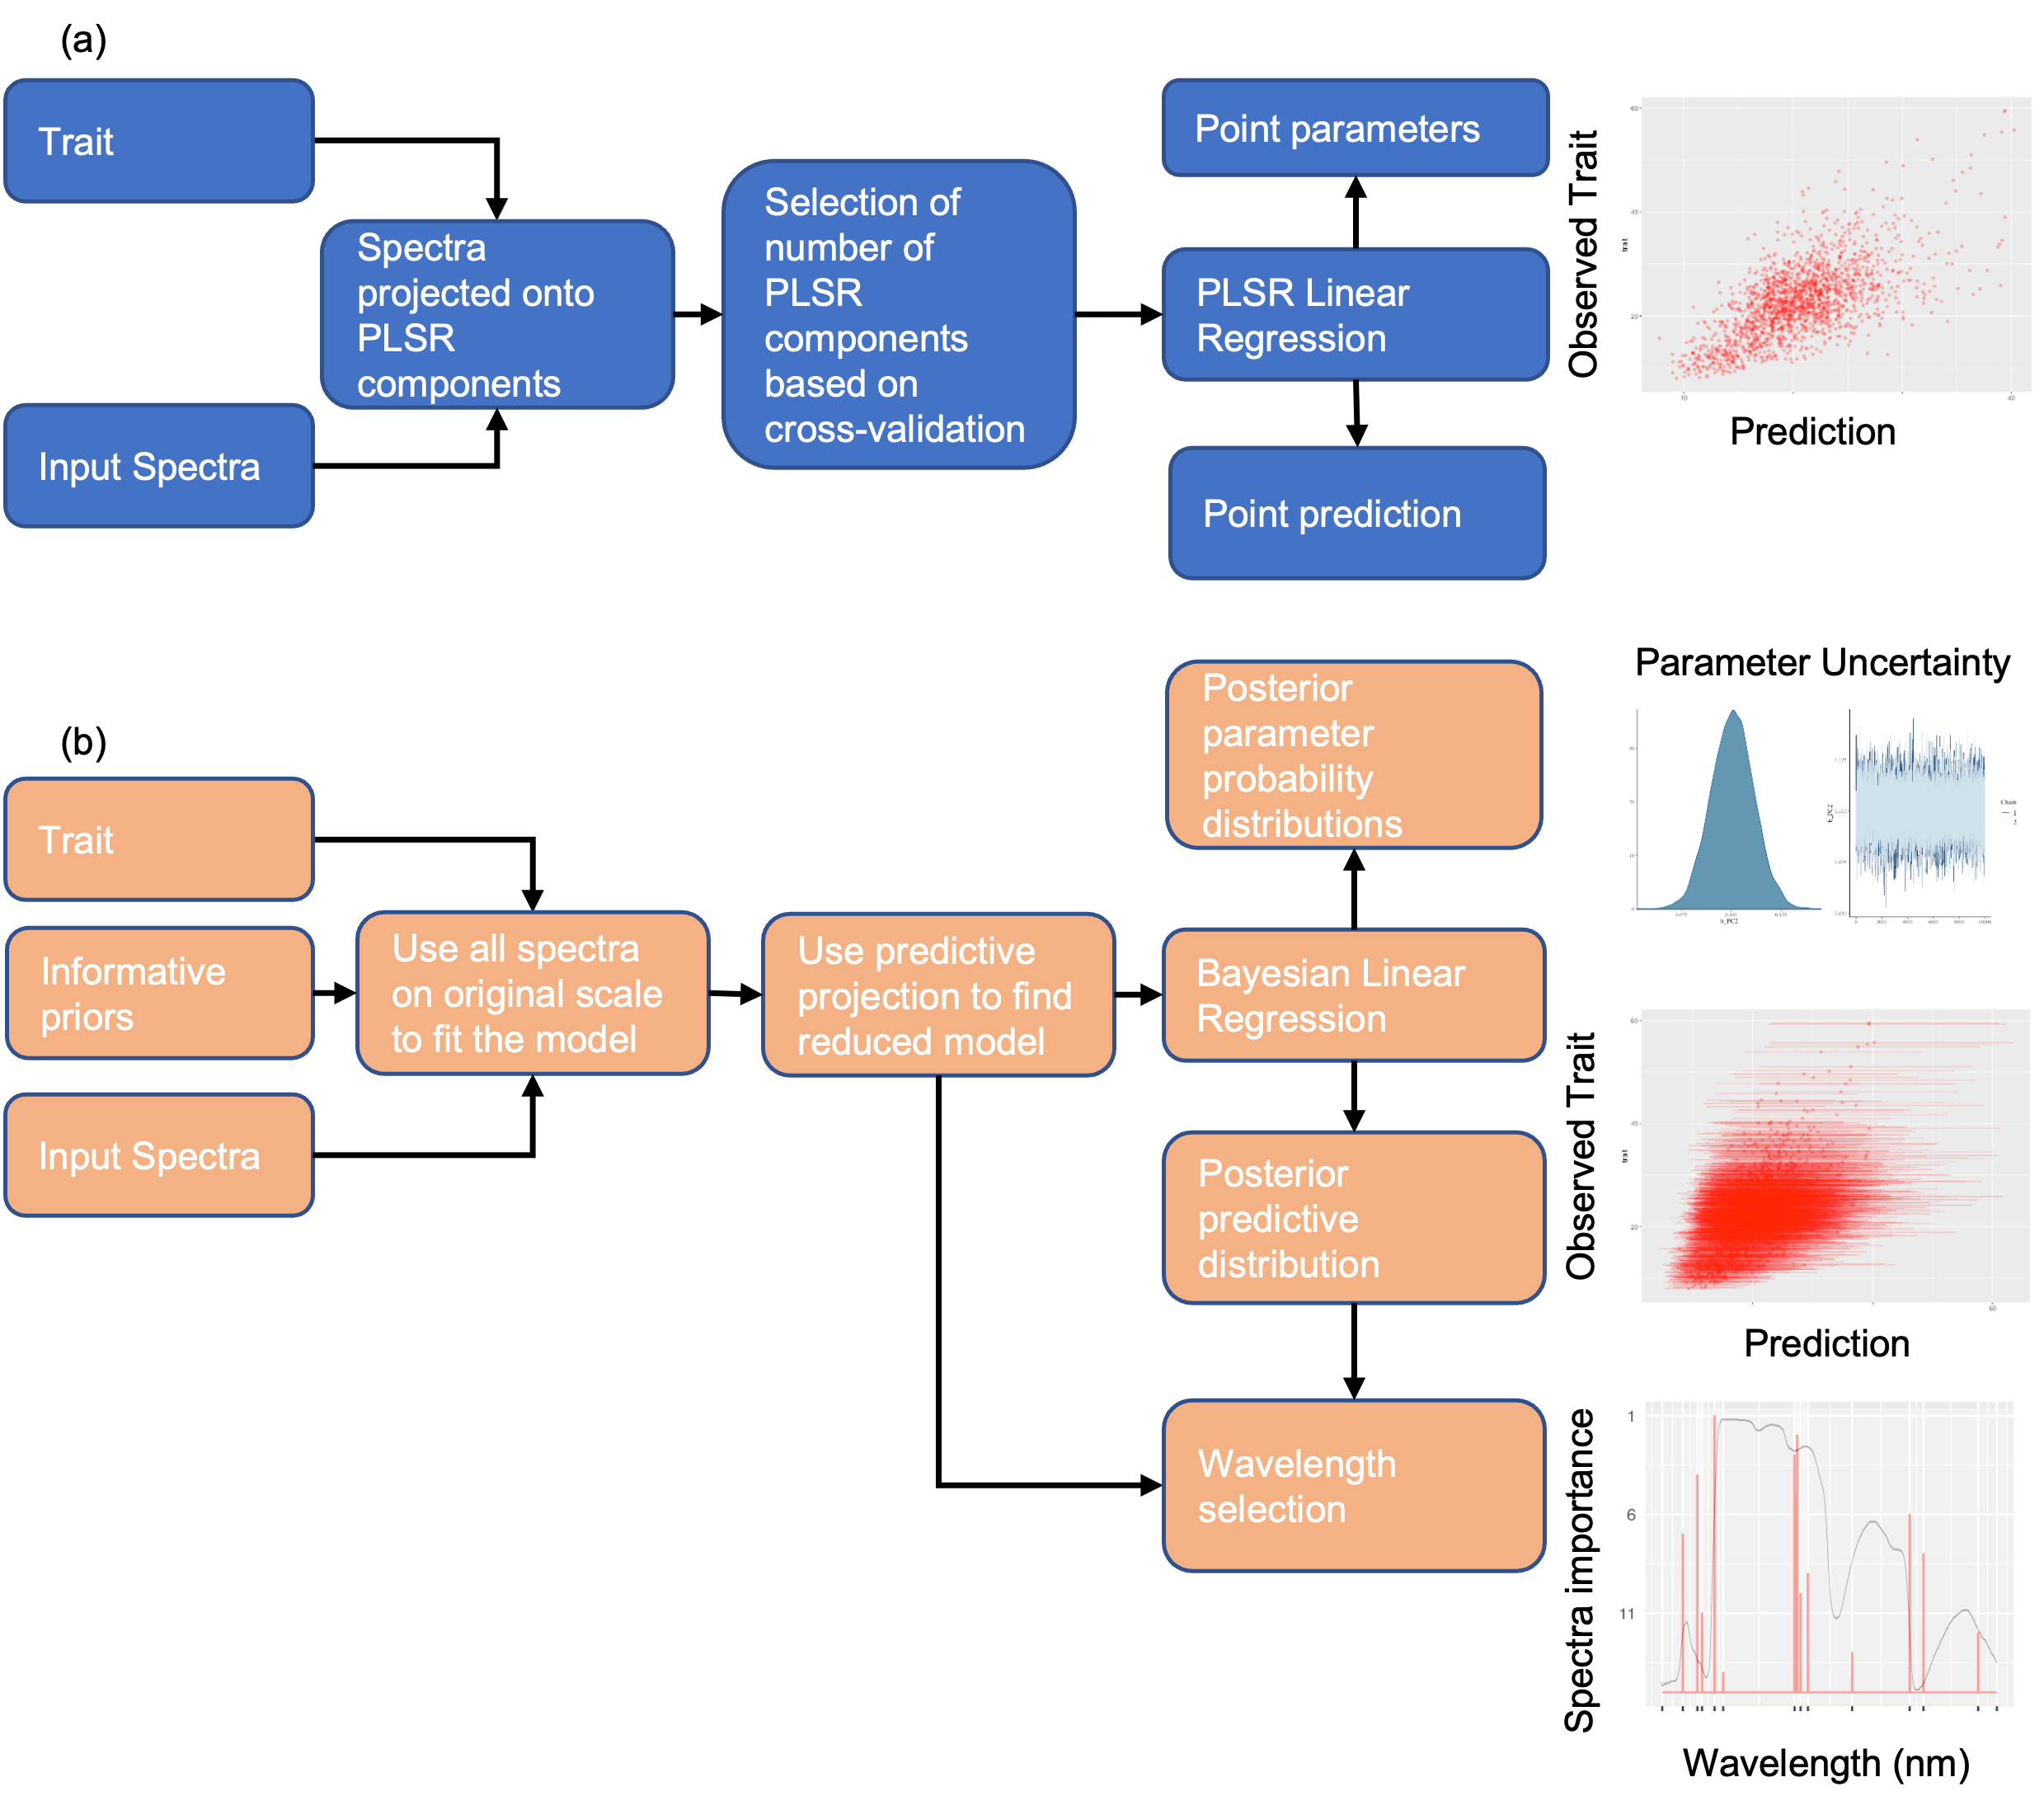
\includegraphics{paper_draft/figures/Method_flowchart.png}

}

\caption{\label{fig-method_flowchart}Comparison between PLSR and the
proposed Bayesian approach}

\end{figure}

\hypertarget{references}{%
\subsection*{References}\label{references}}
\addcontentsline{toc}{subsection}{References}

\hypertarget{refs}{}
\begin{CSLReferences}{1}{0}
\leavevmode\vadjust pre{\hypertarget{ref-arenas-garcia2008}{}}%
Arenas-Garcia, JerÓnimo, and Gustavo Camps-Valls. 2008. {``Efficient
Kernel Orthonormalized PLS for Remote Sensing Applications.''}
\emph{IEEE Transactions on Geoscience and Remote Sensing} 46 (10):
2872--81. \url{https://doi.org/10.1109/TGRS.2008.918765}.

\leavevmode\vadjust pre{\hypertarget{ref-cadotte2009}{}}%
Cadotte, Marc W., Jeannine Cavender-Bares, David Tilman, and Todd H.
Oakley. 2009. {``Using Phylogenetic, Functional and Trait Diversity to
Understand Patterns of Plant Community Productivity.''} \emph{PLOS ONE}
4 (5): e5695. \url{https://doi.org/10.1371/journal.pone.0005695}.

\leavevmode\vadjust pre{\hypertarget{ref-carvalho2010}{}}%
Carvalho, Carlos M., Nicholas G. Polson, and James G. Scott. 2010.
{``The Horseshoe Estimator for Sparse Signals.''} \emph{Biometrika} 97
(2): 465--80. \url{https://www.jstor.org/stable/25734098}.

\leavevmode\vadjust pre{\hypertarget{ref-dupuisVariableSelectionQualitative2003}{}}%
Dupuis, Jérome A., and Christian P. Robert. 2003. {``Variable Selection
in Qualitative Models via an Entropic Explanatory Power.''}
\emph{Journal of Statistical Planning and Inference}, Special issue I:
Model Selection, Model Diagnostics, Empirical Ba yes and Hierarchical
Bayes, 111 (1): 77--94.
\url{https://doi.org/10.1016/S0378-3758(02)00286-0}.

\leavevmode\vadjust pre{\hypertarget{ref-friedlingstein2006}{}}%
Friedlingstein, P., P. Cox, R. Betts, L. Bopp, W. von Bloh, V. Brovkin,
P. Cadule, et al. 2006. {``Climate{\textendash}Carbon Cycle Feedback
Analysis: Results from the C4MIP Model Intercomparison.''} \emph{Journal
of Climate} 19 (14): 3337--53. \url{https://doi.org/10.1175/JCLI3800.1}.

\leavevmode\vadjust pre{\hypertarget{ref-funk2017}{}}%
Funk, Jennifer L., Julie E. Larson, Gregory M. Ames, Bradley J.
Butterfield, Jeannine Cavender-Bares, Jennifer Firn, Daniel C. Laughlin,
Ariana E. Sutton-Grier, Laura Williams, and Justin Wright. 2017.
{``Revisiting the Holy Grail: Using Plant Functional Traits to
Understand Ecological Processes.''} \emph{Biological Reviews} 92 (2):
1156--73. \url{https://doi.org/10.1111/brv.12275}.

\leavevmode\vadjust pre{\hypertarget{ref-goutisModelChoiceGeneralised1998}{}}%
GOUTIS, CONSTANTINOS, and CHRISTIAN P. ROBERT. 1998. {``Model Choice in
Generalised Linear Models: A Bayesian Approach via Kullback-Leibler
Projections.''} \emph{Biometrika} 85 (1): 29--37.
\url{https://doi.org/10.1093/biomet/85.1.29}.

\leavevmode\vadjust pre{\hypertarget{ref-juhopiironenProjectiveInferenceHighdimensional2020}{}}%
Juho Piironen, Markus Paasiniemi, and Aki Vehtari. 2020. {``Projective
Inference in High-Dimensional Problems: Prediction and Feature
Selection.''} \emph{Electronic Journal of Statistics} 14 (1): 2155--97.
\url{https://doi.org/10.1214/20-EJS1711}.

\leavevmode\vadjust pre{\hypertarget{ref-lavorel2002}{}}%
Lavorel, S., and E. Garnier. 2002. {``Predicting Changes in Community
Composition and Ecosystem Functioning from Plant Traits: Revisiting the
Holy Grail.''} \emph{Functional Ecology} 16 (5): 545--56.
\url{https://doi.org/10.1046/j.1365-2435.2002.00664.x}.

\leavevmode\vadjust pre{\hypertarget{ref-pereira2013}{}}%
Pereira, H. M., S. Ferrier, M. Walters, G. N. Geller, R. H. G. Jongman,
R. J. Scholes, M. W. Bruford, et al. 2013. {``Essential Biodiversity
Variables.''} \emph{Science} 339 (6117): 277--78.
\url{https://doi.org/10.1126/science.1229931}.

\leavevmode\vadjust pre{\hypertarget{ref-pettorelli2016}{}}%
Pettorelli, Nathalie, Martin Wegmann, Andrew Skidmore, Sander Mücher,
Terence P. Dawson, Miguel Fernandez, Richard Lucas, et al. 2016.
{``Framing the Concept of Satellite Remote Sensing Essential
Biodiversity Variables: Challenges and Future Directions.''}
\emph{Remote Sensing in Ecology and Conservation} 2 (3): 122--31.
\url{https://doi.org/10.1002/rse2.15}.

\leavevmode\vadjust pre{\hypertarget{ref-piironen2017}{}}%
Piironen, Juho, and Aki Vehtari. 2017. {``Sparsity Information and
Regularization in the Horseshoe and Other Shrinkage Priors.''}
\emph{Electronic Journal of Statistics} 11 (2): 5018--51.
\url{https://doi.org/10.1214/17-EJS1337SI}.

\leavevmode\vadjust pre{\hypertarget{ref-reich2014}{}}%
Reich, Peter B. 2014. {``The World-Wide {`}Fast{\textendash}slow{'}
Plant Economics Spectrum: A Traits Manifesto.''} \emph{Journal of
Ecology} 102 (2): 275--301.
\url{https://doi.org/10.1111/1365-2745.12211}.

\leavevmode\vadjust pre{\hypertarget{ref-serbin2020}{}}%
Serbin, Shawn P., and Philip A. Townsend. 2020. {``Scaling Functional
Traits from Leaves to Canopies.''} In, edited by Jeannine
Cavender-Bares, John A. Gamon, and Philip A. Townsend, 43--82. Cham:
Springer International Publishing.
\url{https://doi.org/10.1007/978-3-030-33157-3_3}.

\leavevmode\vadjust pre{\hypertarget{ref-tranPredictiveLasso2012}{}}%
Tran, Minh-Ngoc, David J. Nott, and Chenlei Leng. 2012. {``The
Predictive Lasso.''} \emph{Statistics and Computing} 22 (5): 1069--84.
\url{https://doi.org/10.1007/s11222-011-9279-3}.

\leavevmode\vadjust pre{\hypertarget{ref-wang2020}{}}%
Wang, Zhihui, Adam Chlus, Ryan Geygan, Zhiwei Ye, Ting Zheng, Aditya
Singh, John J. Couture, Jeannine Cavender-Bares, Eric L. Kruger, and
Philip A. Townsend. 2020. {``Foliar Functional Traits from Imaging
Spectroscopy Across Biomes in Eastern North America.''} \emph{New
Phytologist} 228 (2): 494--511. \url{https://doi.org/10.1111/nph.16711}.

\leavevmode\vadjust pre{\hypertarget{ref-wright2005}{}}%
Wright, Ian J., Peter B. Reich, Johannes H. C. Cornelissen, Daniel S.
Falster, Philip K. Groom, Kouki Hikosaka, William Lee, et al. 2005.
{``Modulation of Leaf Economic Traits and Trait Relationships by
Climate.''} \emph{Global Ecology and Biogeography} 14 (5): 411--21.
\url{https://doi.org/10.1111/j.1466-822x.2005.00172.x}.

\leavevmode\vadjust pre{\hypertarget{ref-wullschleger2014}{}}%
Wullschleger, Stan D., Howard E. Epstein, Elgene O. Box, Eugénie S.
Euskirchen, Santonu Goswami, Colleen M. Iversen, Jens Kattge, Richard J.
Norby, Peter M. van Bodegom, and Xiaofeng Xu. 2014. {``Plant Functional
Types in Earth System Models: Past Experiences and Future Directions for
Application of Dynamic Vegetation Models in High-Latitude Ecosystems.''}
\emph{Annals of Botany} 114 (1): 1--16.
\url{https://doi.org/10.1093/aob/mcu077}.

\end{CSLReferences}



\end{document}
